% !TeX program = xelatex
% Template taken from: Unofficial University of Cambridge Poster Template
% https://github.com/andiac/gemini-cam
% a fork of https://github.com/anishathalye/gemini
% also refer to https://github.com/k4rtik/uchicago-poster

\documentclass[final]{beamer}

% ====================
% Packages
% ====================

\usepackage[T1]{fontenc}
\usepackage{lmodern}
\usepackage[orientation=portrait,size=a0,scale=1]{beamerposter}
\usetheme{gemini}
\usecolortheme{nott}
\usepackage{graphicx}
\usepackage{booktabs}
\usepackage{tikz}
\usetikzlibrary{positioning}
\usetikzlibrary{calc}
\usetikzlibrary{shapes.geometric}  % Required for regular polygons
\usetikzlibrary{decorations.pathmorphing}  % Enables zigzag paths
\usetikzlibrary{decorations.text}
\usetikzlibrary{decorations.markings}
\usetikzlibrary{intersections}
\usetikzlibrary {arrows.meta} 
\usepackage{pgfplots}
\pgfplotsset{compat=1.14}
\usepackage{anyfontsize}
\usepackage{amsmath}
\usepackage{amssymb}
\usepackage[style=vancouver]{biblatex}

\addbibresource{all.bib}

% ====================
% Lengths
% ====================

% If you have N columns, choose \sepwidth and \colwidth such that
% (N+1)*\sepwidth + N*\colwidth = \paperwidth
\newlength{\sepwidth}
\newlength{\colwidth}
\setlength{\sepwidth}{0.025\paperwidth}
\setlength{\colwidth}{0.45\paperwidth}

\newcommand{\separatorcolumn}{\begin{column}{\sepwidth}\end{column}}

% ====================
% Title
% ====================

\title{Analysing the effect of switch positions on power grid stability and development of optimal switch state optimizer}

\author{Sidney Pauly\inst{1} \inst{2}\\ Supervisors: Dr. Nicolas Rubido\inst{1} Dr. Christian Koehler\inst{2}}

\institute[shortinst]{\inst{1} University of Aberdeen \samelineand \inst{2} Venios GmbH}

% ====================
% Footer (optional)
% ====================

\footercontent{
  \href{https://github.com/sidney-pauly}{https://github.com/sidney-pauly} \hfill
  Undergraduate Dissertation Project 2024 \hfill
  \href{mailto:me@sidneypauly.me}{me@sidneypauly.me}}
% (can be left out to remove footer)


% ====================
% Logo (optional)
% ====================

% use this to include logos on the left and/or right side of the header:
\logoright{
\includegraphics[width=8cm]{img/ABDN.png}}
\logoleft{
\includegraphics[width=8cm]{img/venios.png}}

% ==================== 
% Body
% ====================

\begin{document}


\begin{frame}[t]

  \begin{block}{Abstract}
    \textbf{Context}: In modern distribution grids electricity is both produced and consumed on a local level.
    Unlike in the past when energy usually flowed from the transformer to the consumers, nowadays, electricity
    may be produced and consumed within the same grid. This leads to complex powerflow within the distribution
    grids. Venios simulates these grids (in real time) using measurement data, prediction algorithms and whether
    forecasts. Using this "digital twin" of the grid computational studies for improvements of the grid
    can be performed. Improvements desirable for the grid operator might aim at getting a lower overall utilization, higher
    grid stability, lower operating costs or lower expansion costs among others\autocite{Venios}.\\
    \textbf{Aims}: The aim of this project is to explore the effects of connecting or disconnecting different
    sub islands of the grids with each other/from each other. Once these effects are established am algorithm
    finding the optimal switch states can be developed.
  \end{block}

\begin{columns}[t]


\separatorcolumn

\begin{column}{\colwidth}

  \begin{block}{The grid}

    \begin{figure}
      \centering
      \begin{tikzpicture}[scale=7, outer sep=0, inner sep=0,
    nodered/.style={circle, draw=red!60, fill=red!5, very thick, minimum size=2cm},
    nodegreen/.style={circle, draw=green!60, fill=green!5, very thick, minimum size=2cm},
    % nodered/.style={rectangle, draw=red!60, fill=red!5, very thick, minimum size=5mm},
    trianglered/.style={draw,shape=regular polygon,regular polygon sides=3, fill=red!10, minimum size=2.5cm},
    trianglegreen/.style={draw,shape=regular polygon,regular polygon sides=3, fill=green!10, minimum size=2.5cm}
    ]

    % Nodes
    % Grid 2
    \node[trianglered] (trafo1) {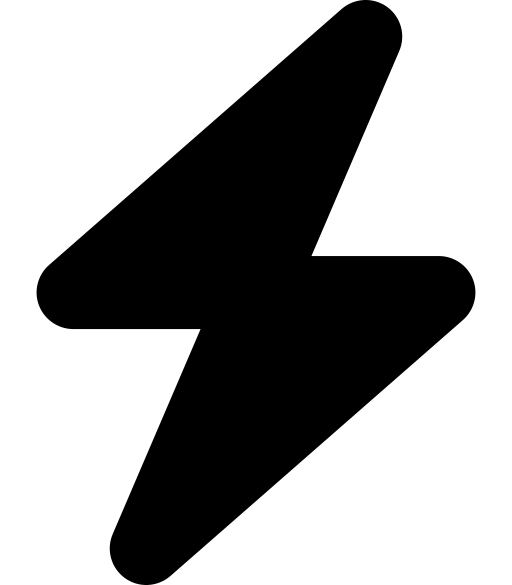
\includegraphics[width=1cm]{img/icons/bolt.png}};
    \node[nodered] (node1_1) [below=of trafo1] {};
    \node[nodered] (node1_2) [left=of node1_1.south west] {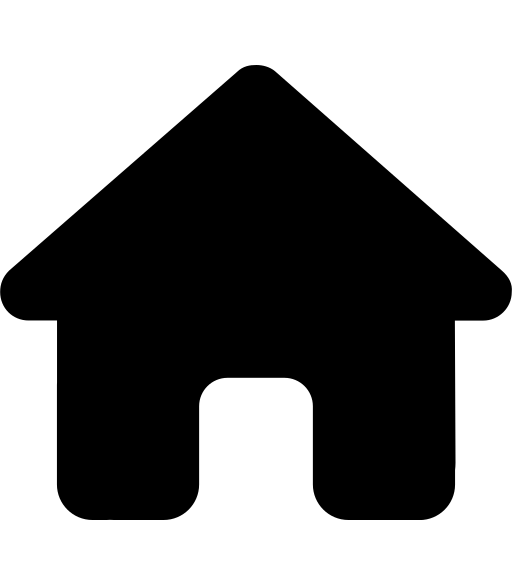
\includegraphics[width=1cm]{img/icons/house.png}};
    \node[nodered] (node1_2a) [below=of node1_1] {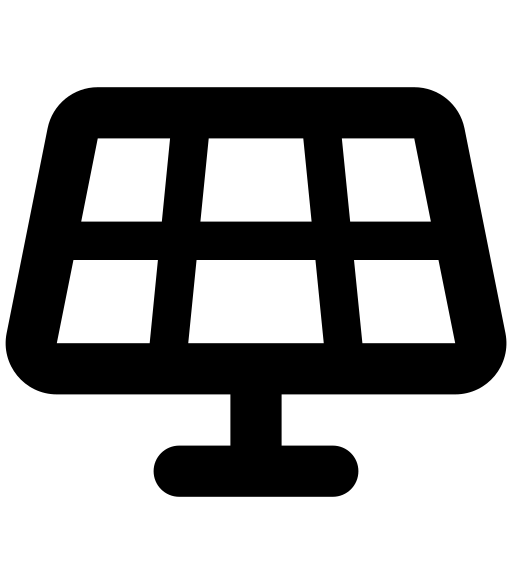
\includegraphics[width=1cm]{img/icons/solar.png}};
    
    \node[nodered] (node1_3) [right=of node1_1] {};
    \node[nodered] (node1_3a) [below=of node1_3] {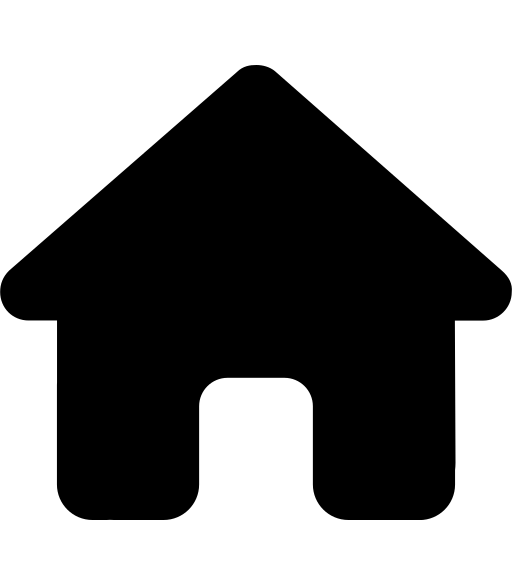
\includegraphics[width=1cm]{img/icons/house.png}};

    \draw[-] (trafo1) -- (node1_1);
    \draw[-] (node1_1) -- (node1_2);
    \draw[-] (node1_1) -- (node1_2a);
    \draw[-] (node1_1) -- (node1_3);
    \draw[-] (node1_3) -- (node1_3a);

    % Grid 2
    \node[nodegreen] (node2_1) [right=3cm of node1_3] {};
    \node[nodegreen] (node2_2) [right=of node2_1] {};
    \node[nodegreen] (node2_2a) at ($(node2_2) + (3mm, -5mm)$)  {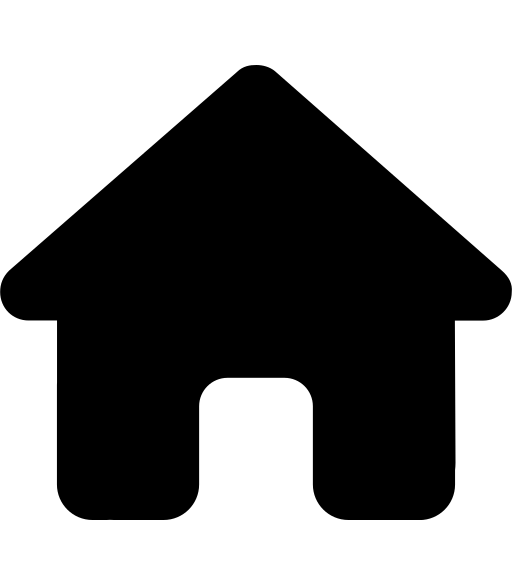
\includegraphics[width=1cm]{img/icons/house.png}};
    \node[nodegreen] (node2_2b) [left=of node2_2a] {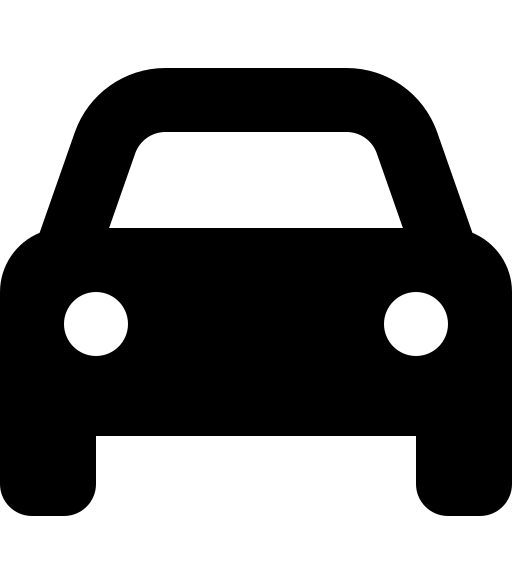
\includegraphics[width=1cm]{img/icons/car.png}};


    \node[nodegreen] (node2_3) [right=of node2_2] {};
    \node[nodegreen] (node2_3a) at ($(node2_3) + (5mm, 3mm)$) {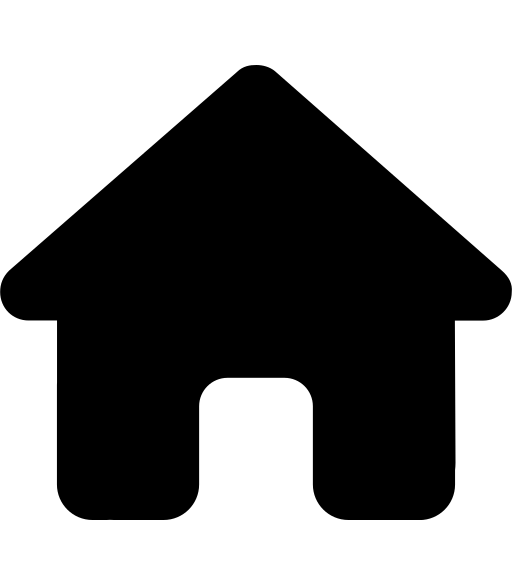
\includegraphics[width=1cm]{img/icons/house.png}};


    \node[nodegreen] (node2_4) at ($(node2_3) + (4mm, -5mm)$) {};
    \node[nodegreen] (node2_4a) at ($(node2_4) + (5mm, 4mm)$) {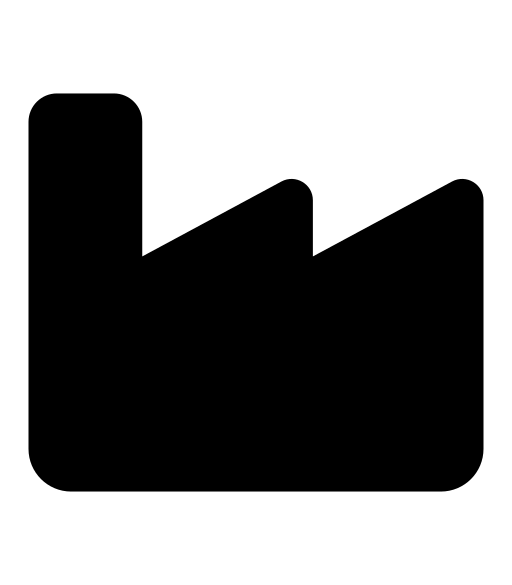
\includegraphics[width=1cm]{img/icons/industry.png}};
    \node[nodegreen] (node2_4b) [below=of node2_4a] {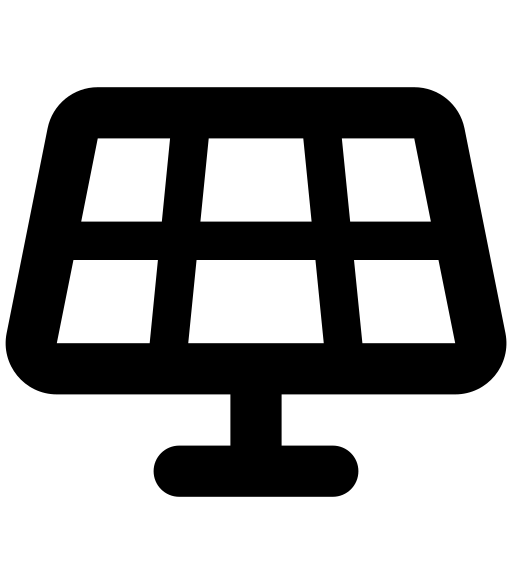
\includegraphics[width=1cm]{img/icons/solar.png}};

    \node[trianglegreen] (trafo2) [above=of node2_2] {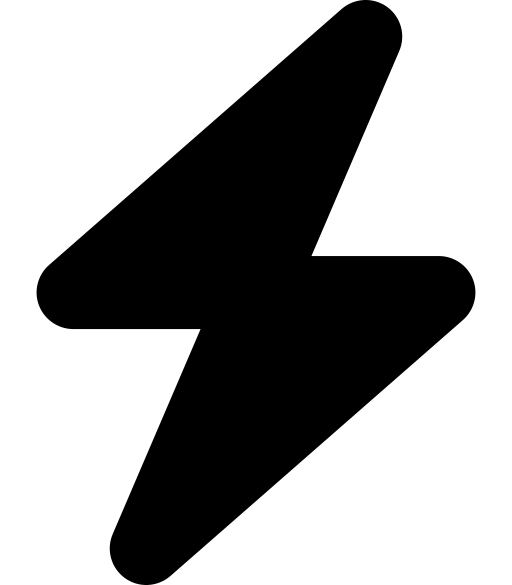
\includegraphics[width=1cm]{img/icons/bolt.png}};
    
    % switch
    \draw[-] (node1_3) -- ([xshift=1.2mm]node1_3.east);
    \draw[-] ([xshift=1.2mm]node1_3.east) -- ([xshift=-1.2mm, yshift=1mm]node2_1.west);
    \draw[-] ([xshift=-1.2mm]node2_1.west) -- (node2_1);

    \draw[-] (trafo2) -- (node2_2);
    \draw[-] (node2_1) -- (node2_2);
    \draw[-] (node2_2) -- (node2_3);
    \draw[-] (node2_3) -- (node2_4);

    \draw[-] (node2_2) -- (node2_2a);
    \draw[-] (node2_2) -- (node2_2b);

    \draw[-] (node2_3) -- (node2_3a);

    \draw[-] (node2_4) -- (node2_4a);
    \draw[-] (node2_4) -- (node2_4b);

\end{tikzpicture}
      \caption{Two electricity grids that are connectable through a switch}
      \label{fig:simple_grid}
    \end{figure}

    A typical distribution grid has many types of prosumers connected like households, industries, solar panels, electric car charges and others.
    Usually all electricity has to come or go to the medium voltage grid through the transformer. However, if the grids are connected
    electricity can flow directly between produces and consumers.

  \end{block}

  \begin{alertblock}{AC Equations}

    \begin{equation}
      \begin{aligned}
          &\text{Voltage:}& \ V(t) &= V_m \cos(\omega t + \theta_V) \\
          &\text{Current:}& \ I(t) &= I_m \cos(\omega t + \theta_I) \\
          &\text{Power:}  & \ P_r(t) &= V(t)I(t)\\
      \end{aligned}
    \end{equation}

    Where $V_m$ and $V_m$ are the magnitudes of voltage and current respectively,
    $\omega$ the angular velocity of the oscillations and $\theta_V$ and $\theta_I$
    the phase offset of Voltage and current respectively.

  \end{alertblock}

  \begin{alertblock}{Complex valued formulation}
    \begin{columns}[t]
      
      \begin{column}{\colwidth/20*5}

        \begin{figure}
          \centering
          \begin{tikzpicture}[scale=4]
            \draw[->, line width=2mm] (-1, 0) -- (1, 1.5);
            \draw[->, line width=2mm] (-1, 0) -- (1, 0); 
            \draw[->, line width=2mm] (1, 0) -- (1, 1.4);  

            \draw[line width=1.5mm] (0, 0) arc (0:45:.8);

            \node[text width=2cm] at (.1, 1.15) {\large $S$};
            \node[text width=2cm] at (1.4, .75) {\large $Q$};
            \node[text width=2cm] at (.2, -.3) {\large $P$};
            \node[text width=2cm] at (-.1, .25) {\large $\theta$};

          \end{tikzpicture}
        \end{figure}

      \end{column}

      \begin{column}{\colwidth/10*6}

        \begin{equation}
          \begin{aligned}
              &\text{Complex power:}    &S       &= P + i Q\\
              &\text{Apparent power:}   &|S|     &= |V||I| = V_m I_m\\
              &\text{Impedance Angle:}  &\theta  &= \theta_V-\theta_I \\
              &\text{Active (real part):}     &P       &= |V||I| \cos{\theta} = V_m I_m\cos{\theta} \\
              &\text{Reactive (imaginary part):}   &Q       &= |V||I| \sin{\theta} = V_m I_m\sin{\theta}\\
              &\text{Power factor:}     &P_f     &= \cos{\theta}
          \end{aligned}
        \end{equation}
      \end{column}

    \end{columns}
  \end{alertblock}

  \begin{block}{Powerflow}
    

    Solving power flow means figuring out the voltage at each node and the
    current flowing into it.

    \begin{columns}[t]
      
    \begin{column}{\colwidth/20*7}

      \begin{figure}
        \centering
        \begin{tikzpicture}[scale=4]

    % Bus
    \draw[line width=1mm] (0, 0) -- (0, 2) node(bus)[above]{$V_i \ (\text{bus node})$};

    % Current Incoming  
    \draw[->, line width=1mm] (-.3, .6) to [edge label=\large $I_i$] ++(.2,0) coordinate(p);
    \draw[-, line width=1mm] (p) -- (p -| bus);

    % Load
    \draw[-, line width=1mm] (0, .2) -- ++(.4, 0) coordinate(p);
    \draw[-, line width=1mm] (p) -- ++(0, -.4) coordinate(p);
    \draw[line width=1mm]  ($(p) - (.15, 0)$) rectangle ++(.3, -.5) coordinate(l);
    \node[line width=1mm] (lLabel) at (l)[right] {$y_{i0}$}; %label
    \draw[line width=1mm] ($(p) - (0, .5)$) -- ++(0, -.2) coordinate(p);
    \draw[line width=1mm] ($(p) + (-.2, 0)$) -- ($(p) + (.2, 0)$);
    \draw[line width=1mm] ($(p) + (-.15, -.1)$) -- ($(p) + (.15, -.1)$);
    \draw[line width=1mm] ($(p) + (-.1, -.2)$) -- ($(p) + (.1, -.2)$);

    % Other nodes
    \draw[line width=1mm] (1, 1.7) coordinate(s) to [edge label=\large $y_{i1}$] (s -| bus) coordinate(p);
    \draw[line width=1mm] ($(s) + (0, .1)$) -- ($(s) + (0, -.1)$);
    \node (label) at (s)[above] {$V_1$};

    \draw[line width=1mm] (1.5, 1.2) coordinate(s) to [edge label=\large $y_{i2}$] (s -| bus) coordinate(p);
    \draw[line width=1mm] ($(s) + (0, .1)$) -- ($(s) + (0, -.1)$);
    \node (label) at (s)[above] {$V_2$};

    \draw[line width=1mm] (2, .4) coordinate(s) to [edge label=\large $y_{in}$] (s -| bus) coordinate(p);
    \draw[line width=1mm] ($(s) + (0, .1)$) -- ($(s) + (0, -.1)$);
    \node (label) at (s)[above] {$V_n$};

  \end{tikzpicture}
        \caption{Schematic of a powerflow node\autocite{power_system_analysis}}
      \end{figure}

    \end{column}

    \begin{column}{\colwidth/20*12}

      \begin{equation}
        \begin{aligned}
          &\text{Reistance}: \ \ & R\\
          &\text{Reactance}: \ \ & X\\
          &\text{Impedance}: \ \ & Z   &= R + iX\\
          &\text{Admittance}:\ \ & Y   &= 1/Z = \begin{pmatrix}y_{11}&y_{12}&...&y_{1n}\\y_{21}&...&&\\...&&...&\\y_{n1}&&&y_{nn}\\\end{pmatrix}\\
          &\text{Ohm's law}: \ \ & V   &= Z I \\
          &\text{Powerflow}: \ \ & I_i &= V_i \sum_{j=0}^n y_{ij} - \sum_{j=1}^n y_{ij} V_j = \frac{S_i^*}{V_i^*} \quad i \neq j
        \end{aligned}
      \end{equation}
      
    \end{column}

  \end{columns}

  \vspace{1cm}

  To solve power flow each node in the grid is modelled as one of two types:

  \begin{center}
    \begin{tabular}{ llll } 
     Name & Known       & Example                     & Number \\ 
     \hline
     Slack& $V$         & Transformer or big prosumer & One\\
     PQ   & $P$ \& $Q$  & Any prosumer                & Any\\
    \end{tabular}
  \end{center}

  This results in a system of equations, as $V_i$ appears on both sides it is non-linear and
  can only be solved computationally

  \end{block}


  \begin{block}{Interacting with VEP}

    \begin{figure}
      \centering
      \begin{tikzpicture}[scale=2]

        \node[draw, fill=black] (vep)  {
\includegraphics{img/venios.png}};

        \node(topology)    [left=of vep]   {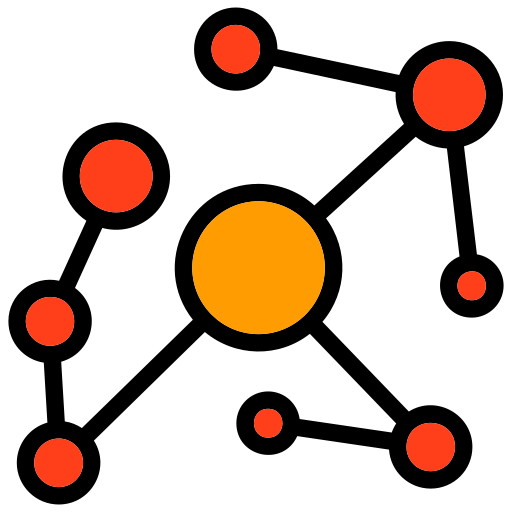
\includegraphics[width=2cm]{img/icons/knowledge-graph.png}};
        \node             [below= 1mm of topology]   {Topology};

        \node(load)    [below=1cm of topology]   {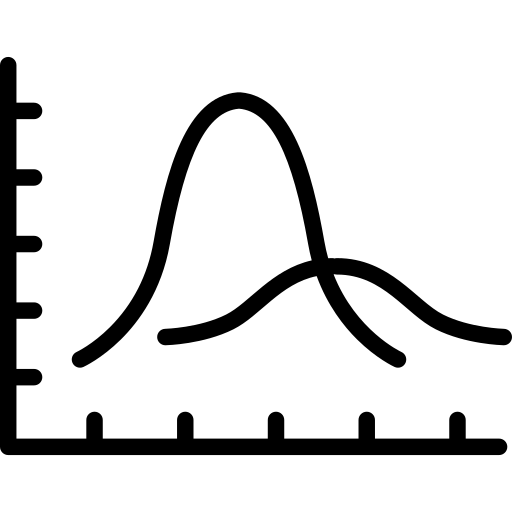
\includegraphics[width=2cm]{img/icons/wave-graph.png}};
        \node             [below= 1mm of load]   {Load Profiles};

        \node(weather)    [left=3cm of load]   {
\includegraphics[width=2cm]{img/icons/sun.png}};
        \node             [below= 1mm of weather]   {Weather Data};

        \node(phys_limits)    [above=1cm of topology]   {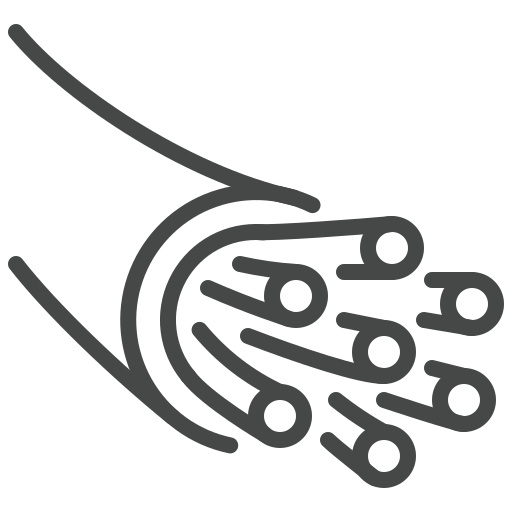
\includegraphics[width=2cm]{img/icons/internet.png}};
        \node             [below= 1mm of phys_limits]   {Physical Limits};

        \node(op_limits)    [left=3cm of phys_limits]   {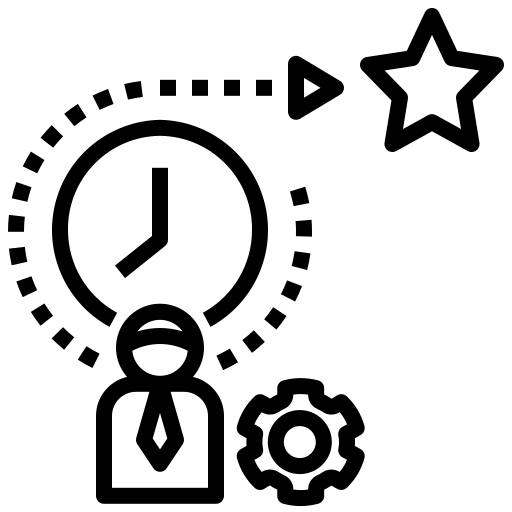
\includegraphics[width=2cm]{img/icons/long-term.png}};
        \node             [below= 1mm of op_limits]   {Op. Limits};

        % \draw[->] (topology) -- (vep);
        % \draw[->] (phys_limits) -- (vep);
        % \draw[->] (op_limits) -- (vep);
        % \draw[->] (load) -- (vep);
        % \draw[->] (weather) -- (vep);

        \node(my_module)    [right=5cm of vep]   {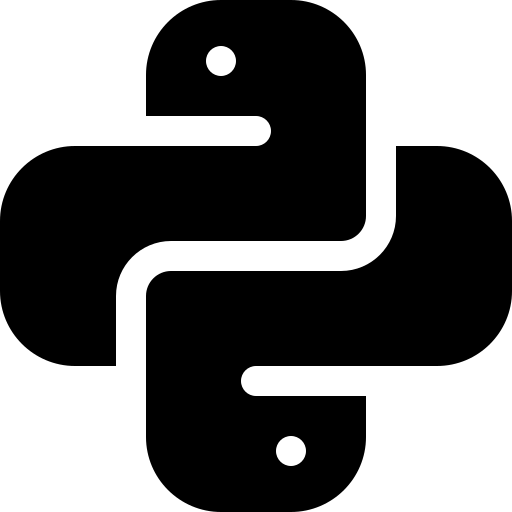
\includegraphics[width=2cm]{img/icons/python.png}};
        \node             [below= 1mm of my_module]   {Optimizer};

        \node(c_kernel)    [right=1cm of my_module]   {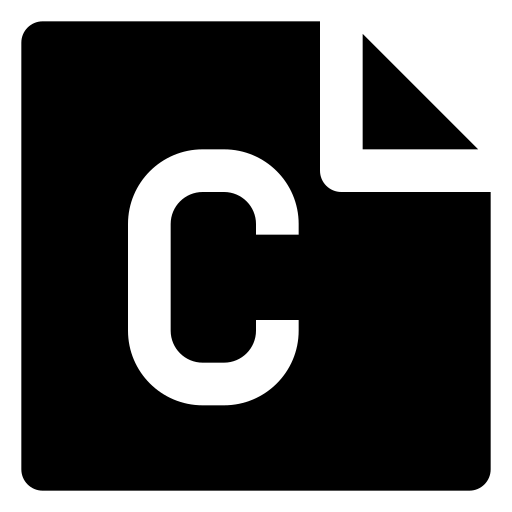
\includegraphics[width=2cm]{img/icons/c-file.png}};
        \node             [below= 1mm of c_kernel]   {Powerflow};

        \draw [-{Latex[length=5mm]}, line width = 1mm] (vep.north) to [bend left=30, edge label=Api] (my_module.north west);
        \draw [-{Latex[length=5mm]}, line width = 1mm] (my_module.south west) to [bend left=30, edge label=Optimal switch state] (vep.south);


      \end{tikzpicture}
    \end{figure}

  \end{block}


\end{column}

\separatorcolumn

\begin{column}{\colwidth}

  \begin{block}{Solving powerflow}
    
    \begin{itemize}
      \item \textbf{Gauss Seidel}: Easy to implement, but slow and bad convergence
      \item \textbf{Newton Raphson}: More complex, but very fast
    \end{itemize}
  
  
    \begin{columns}[t]
        
      \begin{column}{\colwidth/20*9}
  
        \begin{figure}
          \centering
          \begin{tikzpicture}[scale=4]

    \newcommand*{\eq}{=}
    \newcommand*{\interceptpos}{3.05}

    % Axis
    \draw[->,thick, line width=.7mm, name path=xaxis] (-.5,0) -- (4,0) coordinate(xlbl);
    \draw[->,thick, line width=.7mm] (0,-.5) -- (0,2.5);

    % fx
    \clip (-.7, -.7) rectangle (4, 2.5);
    \draw[
        -,
        blue,
        domain=-.5:4,
        smooth,
        line width=1mm,
        variable=\x,
        name path=fx
    ] plot ({\x},\x*\x*.2 -.3);

    \filldraw[
        red, 
        name intersections={of=fx and xaxis}
    ] (intersection-1) coordinate(x) circle (.5mm);

    \node at (x)[below] {$x$};

    % Tangent
    \draw[
        -,
        domain=-.5:4,
        smooth,
        line width=.9mm,
        variable=\x,
        black,
        name path=tangent
    ] plot({\x},{2*\interceptpos*.2*(\x - \interceptpos) + (\interceptpos*\interceptpos*.2 -.3)});

    \filldraw[
        red, 
        name intersections={of=tangent and xaxis}
    ] (intersection-1) coordinate(x1) circle (.5mm);

    \node at (x1)[below] {$x_1$};

    % Intercept
    \path[name path=intercept] (\interceptpos, 0) coordinate(x0) -- ++(0, 4);
    \draw[
        dotted, 
        line width=1mm,
        name intersections={of=fx and intercept}
    ] (x0) to [edge label= $\Delta y \eq f(x)$, sloped] (intersection-1) coordinate(v0);

    \filldraw [red] (x0) circle (.5mm);
    \filldraw [red] (v0) circle (.5mm);

    \node at (x0)[below] {$x_0$};
    \node at (v0)[left] {$f(x_0)$};

    \draw[<->, line width=1mm,name path=dx] ($(x1) - (0, .4)$) -- ($(x0) - (0, .4)$) node[pos=0.5](dxlbl){};

    \node at (dxlbl)[below]{$\Delta x$};

    % Formula

    \node[draw, fill=white] at (.5, 1) { $x_1 \eq x_0 - \frac{f(x_0)}{f'(x_0)}$ };


  \end{tikzpicture}
          % \caption{Illustration of Newton Raphson method for simple fuction}
        \end{figure}
  
      \end{column}
  
      \begin{column}{\colwidth/20*9}
  
        \begin{figure}
          \centering
          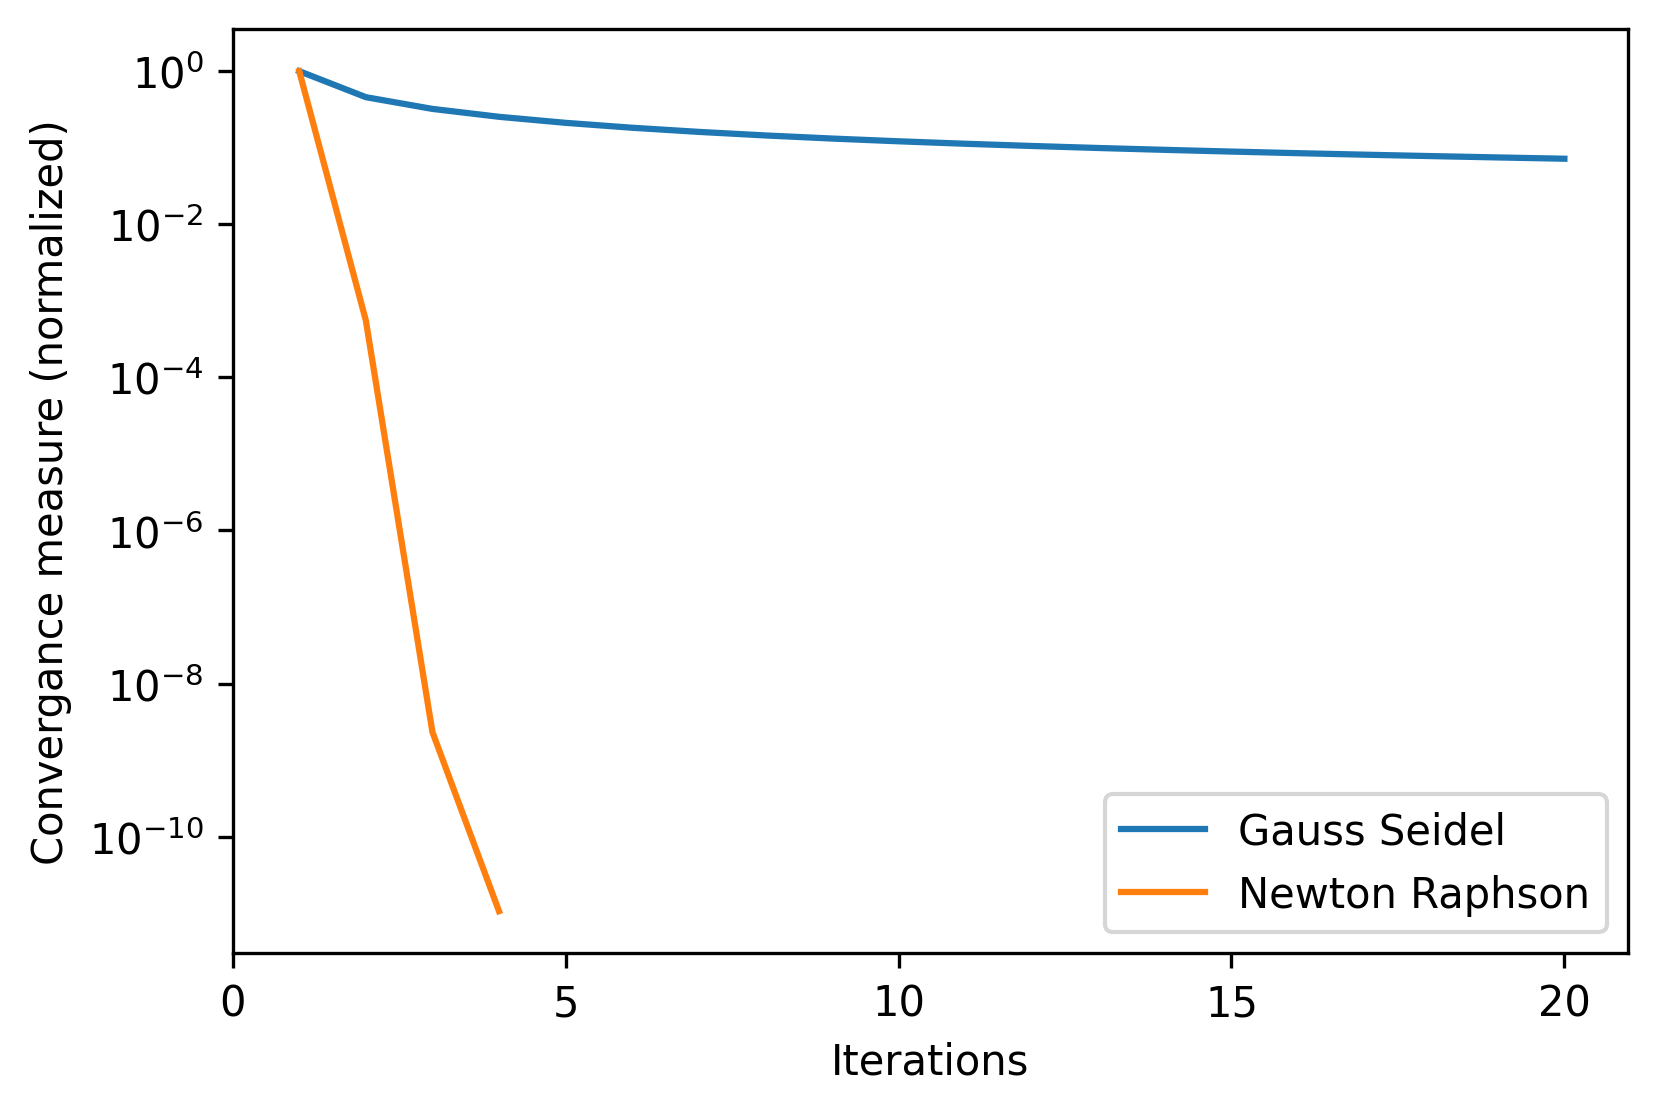
\includegraphics[width=18cm]{./img/graphs/convergance.png}
          % \caption{Comparing Gauss Seidel and Newton Raphson powerflow convergance}
        \end{figure}
  
      \end{column}
  
    \end{columns}

 \end{block}

 \begin{block}{Powerflow result}

  \begin{figure}
    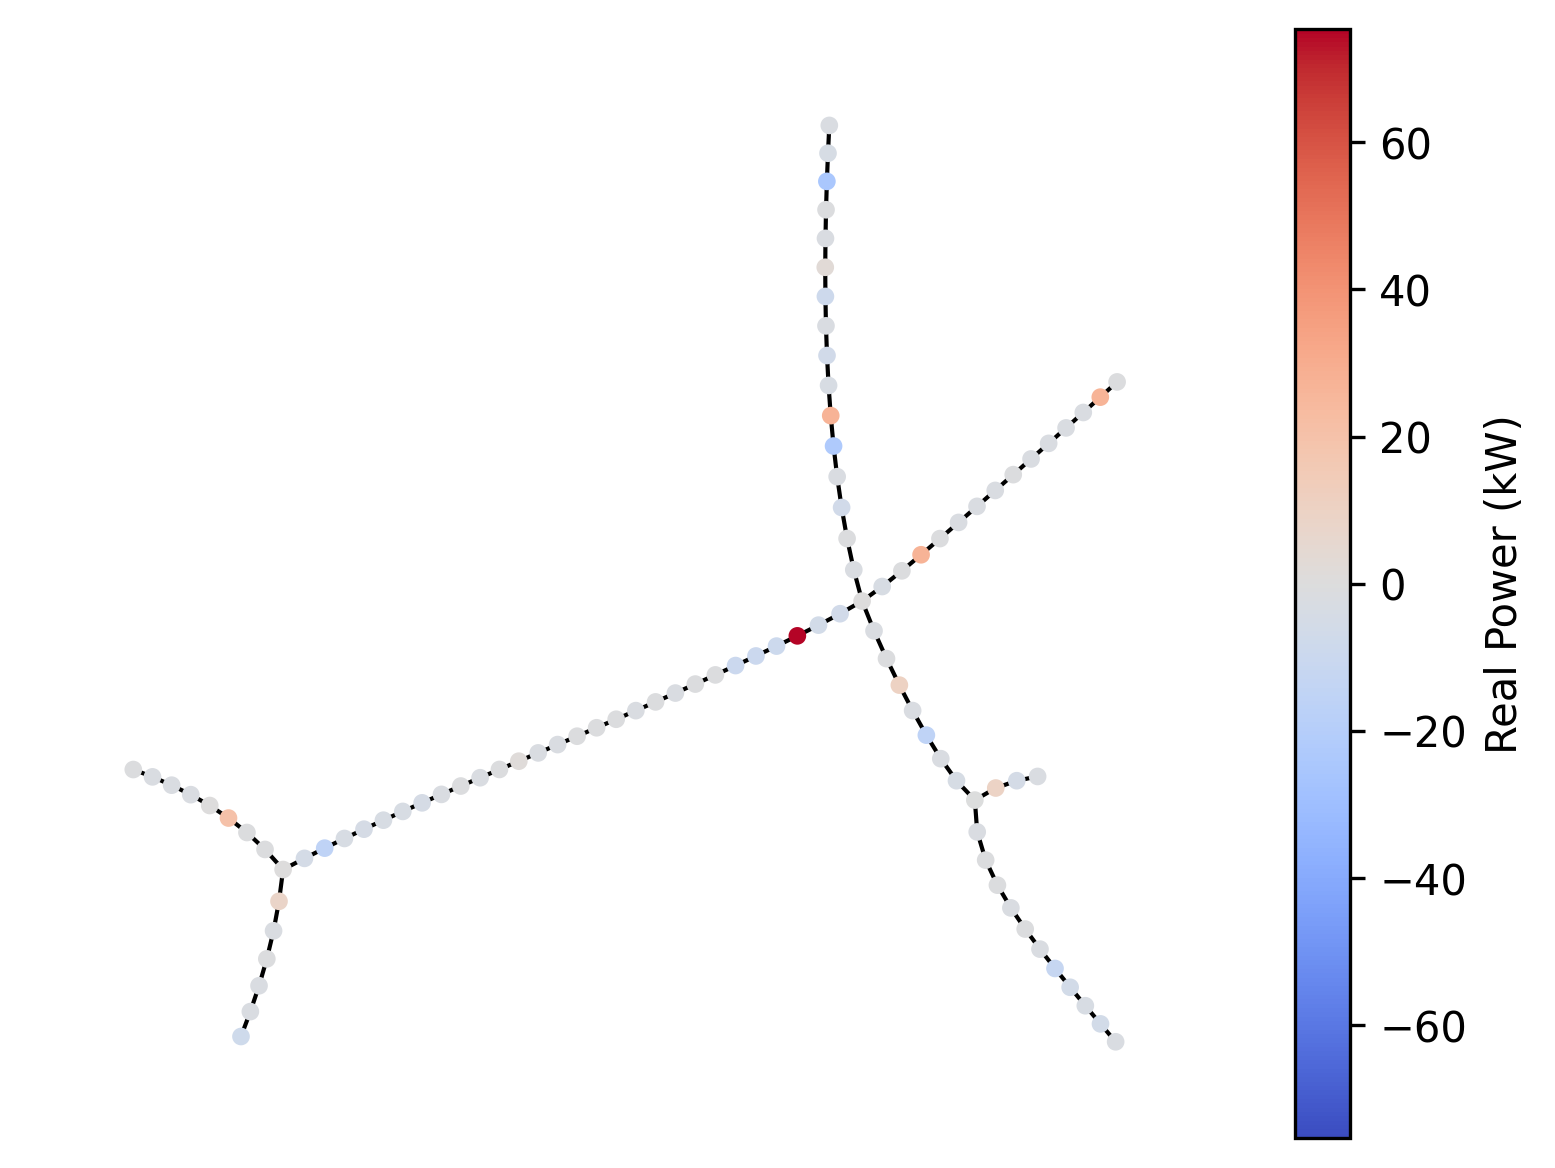
\includegraphics[width=.48\textwidth]{img/graphs/rural1/power.png}\hfill
    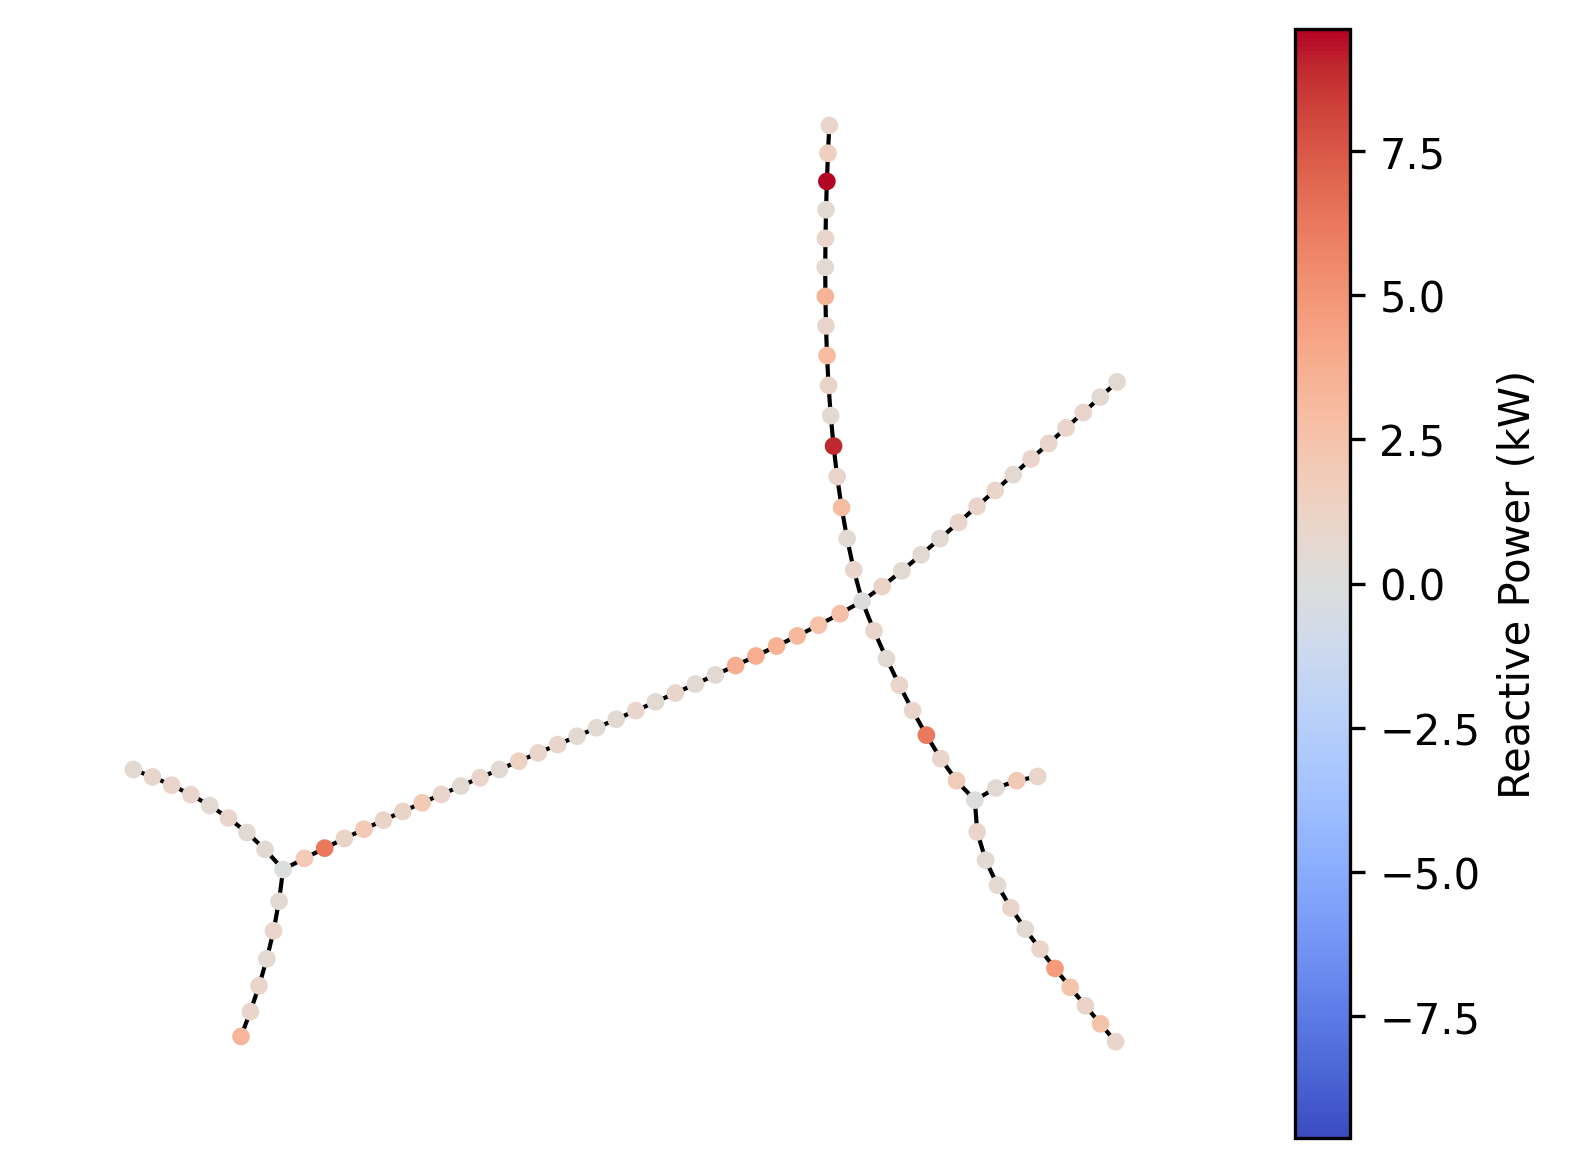
\includegraphics[width=.48\textwidth]{img/graphs/rural1/power_react.png}\hfill
    \\[\smallskipamount]
    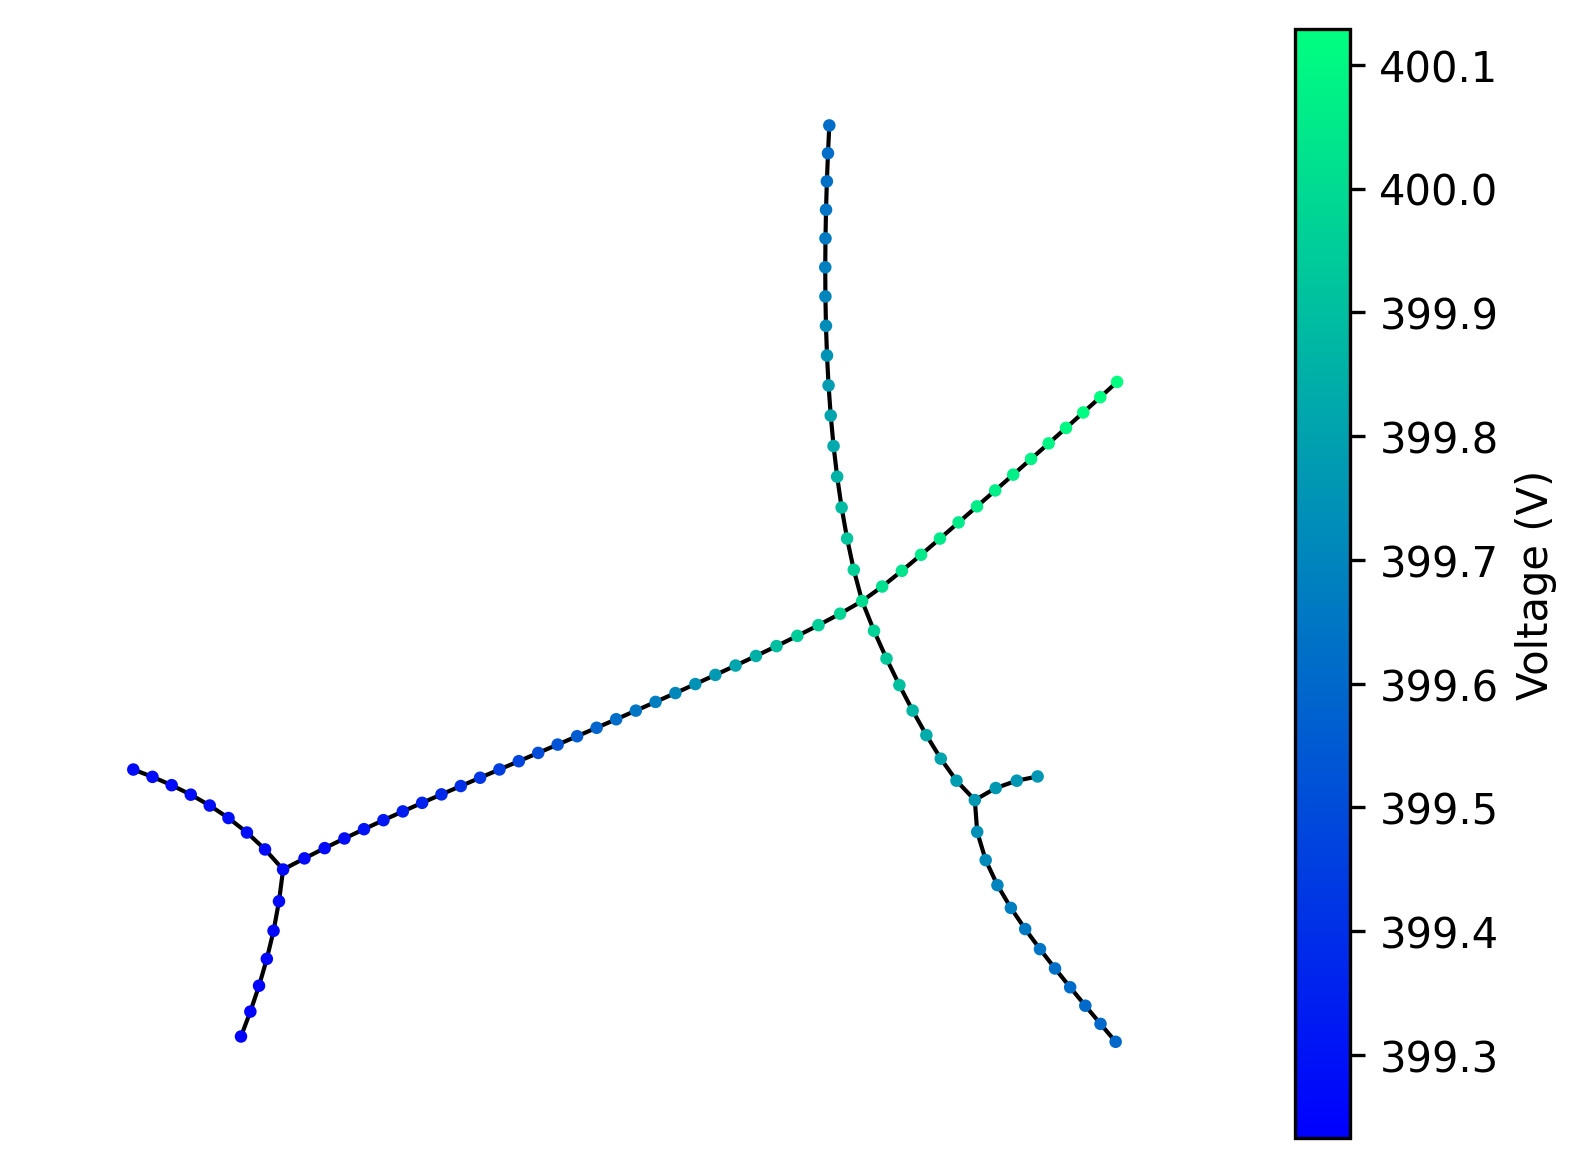
\includegraphics[width=.48\textwidth]{img/graphs/rural1/voltage.png}\hfill
    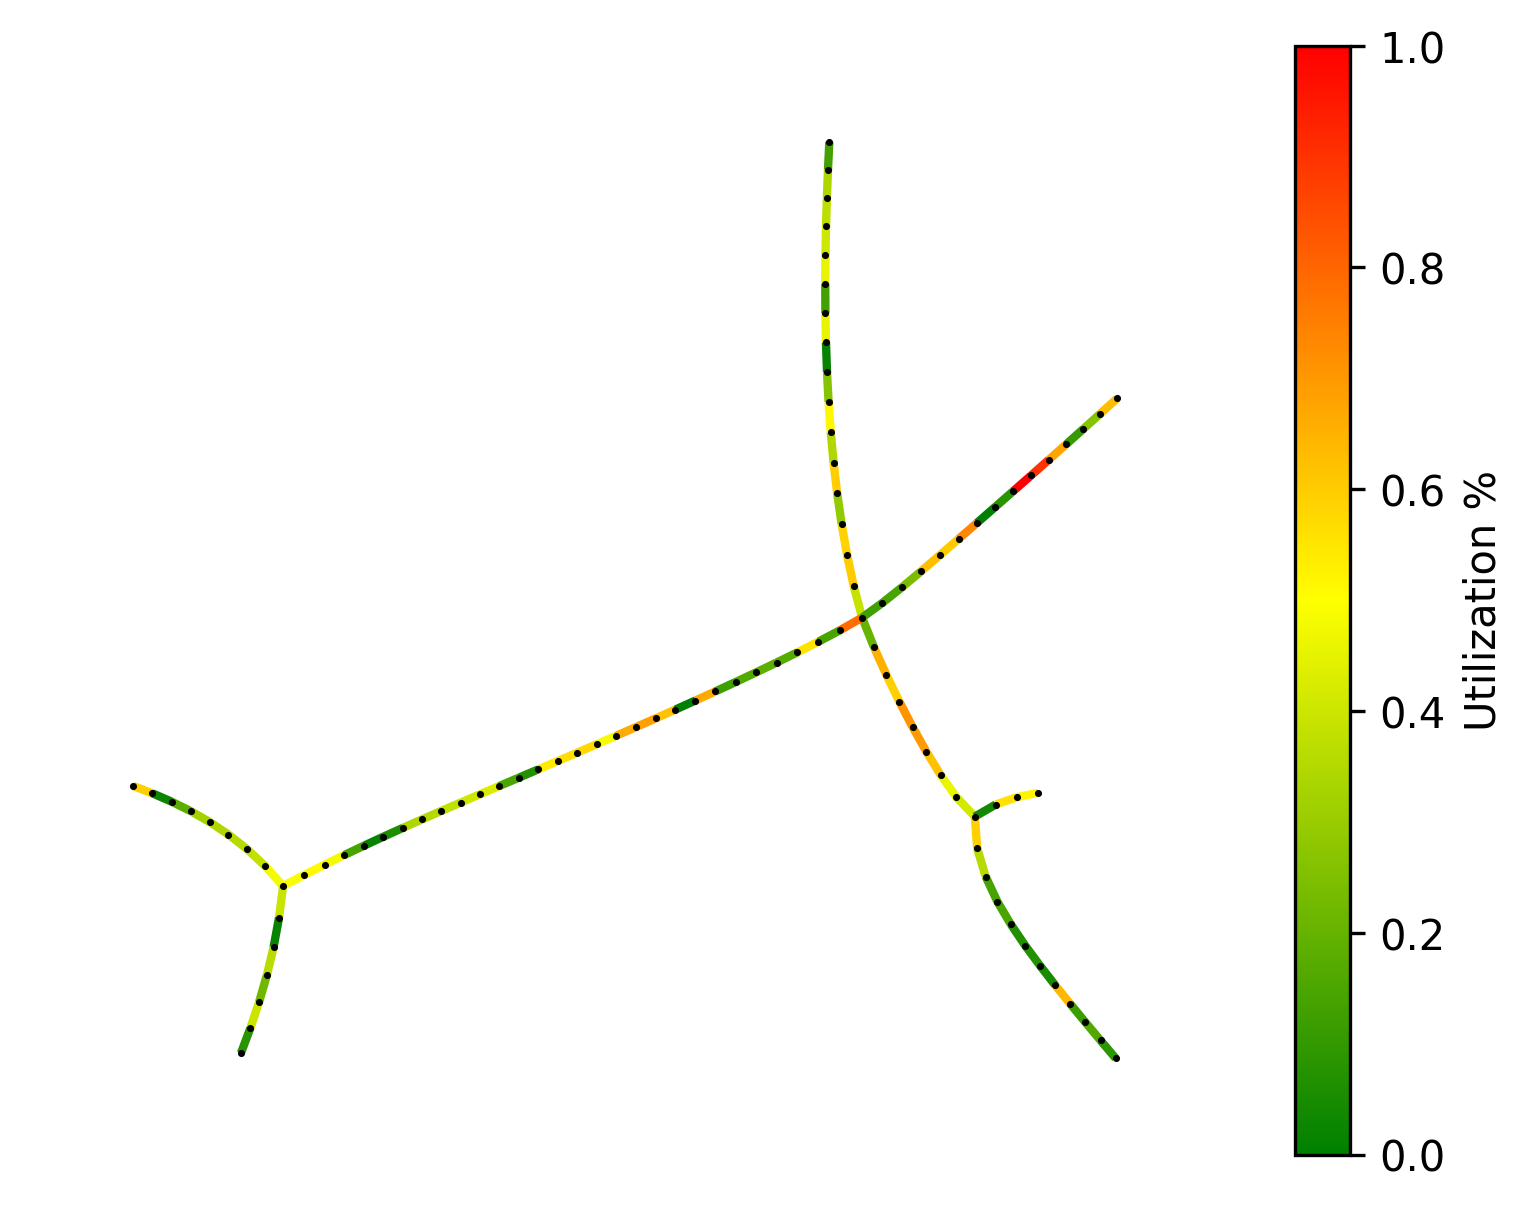
\includegraphics[width=.48\textwidth]{img/graphs/rural1/cable_utilization.png}\hfill
    \caption{Results of powerflow simulation of SimBench Grid "1-LV-rural1"\autocite{en13123290} using Newton Raphson }\label{fig:foobar}
  \end{figure}  

 \end{block}

  \begin{exampleblock}{Typical German urban grid}

    \begin{columns}[t]
        
      \begin{column}{\colwidth/20*7}

        \begin{equation*}
          \begin{aligned}
           \large \text{Switch states} = 2^{\text{Number switches}}
          \end{aligned}
        \end{equation*}


      \end{column}

      \begin{column}{\colwidth/20*11}
        \begin{itemize}
          \item $~100-1000$ Prosumers per grid\autocite{Venios}
          \item $~1-4$ connections to neighbouring grids\autocite{Venios}
          \item City of 500.000 people tends to have $~1000$ grids\autocite{Venios}
          \item High percentage of households/industries generating power
        \end{itemize}
      \end{column}

    \end{columns}
    
    
  \end{exampleblock}

 \begin{block}{Outlook}
 
  To find optimal (or even improved switch states), two challenges need to be: what
  does \textit{improved} mean and which configurations should be considered?

  \begin{columns}[t]
          
    \begin{column}{\colwidth/20*7}

      % \begin{block}{Measures to asses grid quality}
      \textbf{Measures to assess grid quality:}
    
        \begin{itemize}
          \item Overall line losses
          \item Utilization of cables
          \item Utilization of transformers
          \item Number of trafos
          \item Voltage stability
          \item Expandability robustness
        \end{itemize}
    
      % \end{block}

    \end{column}

    \begin{column}{\colwidth/20*11}
      
      \textbf{Switching Strategies:}

      % \begin{block}{Switching Strategies}
        \begin{itemize}
          \item Quantify how different two configurations are and pick very different ones
          \item Use centrality measures
          \item Balance the number of nodes or the load sum of nodes connected to one transformer
          \item Bad apple
          \item Random
          \item Determine typical grid topologies
        \end{itemize}
    
      % \end{block}
    \end{column}

  \end{columns}

\end{block}

  


 

  \begin{block}{References}

    \printbibliography

    % \nocite{*}
    % \footnotesize{\bibliographystyle{plain}\bibliography{poster}}

  \end{block}

\end{column}

\separatorcolumn

\end{columns}

\end{frame}


\end{document}


% Notes: 
%1. Add Ohms law to explain how to get to pf formulation
%2. Structure as model, methods and results
